\chapter{Outcome and further work}

In this chapter the main concerns are listed.
For each concern the current progress is described as well as further work that needs to be done.


\todo{. old sections}

\section{Storage}

One of the central concerns is the storage management.
The program needs to make input files available on each execution node and collect the results once the computation is complete.
There are a few main architectural strategies to approach this.
Simplified, either at a centralized location which is accessed by all execution nodes, a copy of the input files to the execution nodes or decentralized and distributed between all execution nodes and replication.
The advantages and disadvantages can depend on the specific implementation and is therefore discussed in combination of such (see \autoref{state_of_the_art}).

Further testing is required to decide whether a more complex storage system is required, or the simplicity of a centralized solution outweighs the setup and maintenance overhead.

%\subsection{Hadoop File System}
%\cite{hdfs:main}
%\cite{hdfs:doc}
%\todo{redudancy for evenly distributed}

%\subsection{NFS}
%
%local/per node cache?

\section{Coordination}

Another important concern is the coordination of the nodes.
A central coordinator with external server nodes, such as GitLab and Jenkins have, might not be sufficient for more complex and longer lasting pipelines.
The probability that the master would need to be offline while there is a stage executed, is in the scenario of the desired workflow higher than for GitLab or Jenkins, because the stage is being execution for hours or days.
Coupling stage execution plans on node availability ahead of time, as well as recovering from a sudden master failure implies additional implementation complexity.
A decentralized coordination needs to be able to do this as well, but also allows the usage of the system while a node failed or is unreachable due to maintenance.
With further prototyping and research a reasonable solution shall be found.

\section{Binary distribution}

In a time where containers are common and have proven to be usable, the installation of the binaries directly on the operating system they are executed on shall be avoided.
There shall be no manual, nor automatic but custom file copies of the binaries or images from one server to the other.
Experience shows, that without a proper management, this can easily become a mess, in which it is no longer clear, which files or images belong to which version.
At the same time, making all binaries publicly available through the Docker Hub\cite{docker:hub} is no option either.
Whether a self hosted Docker Registry\cite{docker:registry} could be the solution to this will be determined in further testing.

\section{User Interface}

Providing a useful user interface might not be important to the functionality of the system itself but for the user experience.
A bad user experience will cause a system not to be used.
It became common practice for a rich user experience to be web based and interactive with JavaScript.
For a potentially decentralized system, it is also advantageous to be able to access a disconnected node in the same manner as the remaining system, which further encourages a web based solution.
Web based solutions such as React and Angular shall therefore be investigated for being used as user interface.

\section{Requirements}

\todo{more than first defined - as expected}

\todo{lots more UI shortcuts found necessary while starting to use winslow}

\section{Architecture}

\todo{loosely coupled backend driver}\autoref{architecture:detailed}

\section{High Level System Overview}


\todo{intro words}

\begin{figure}[h]
	\centering
	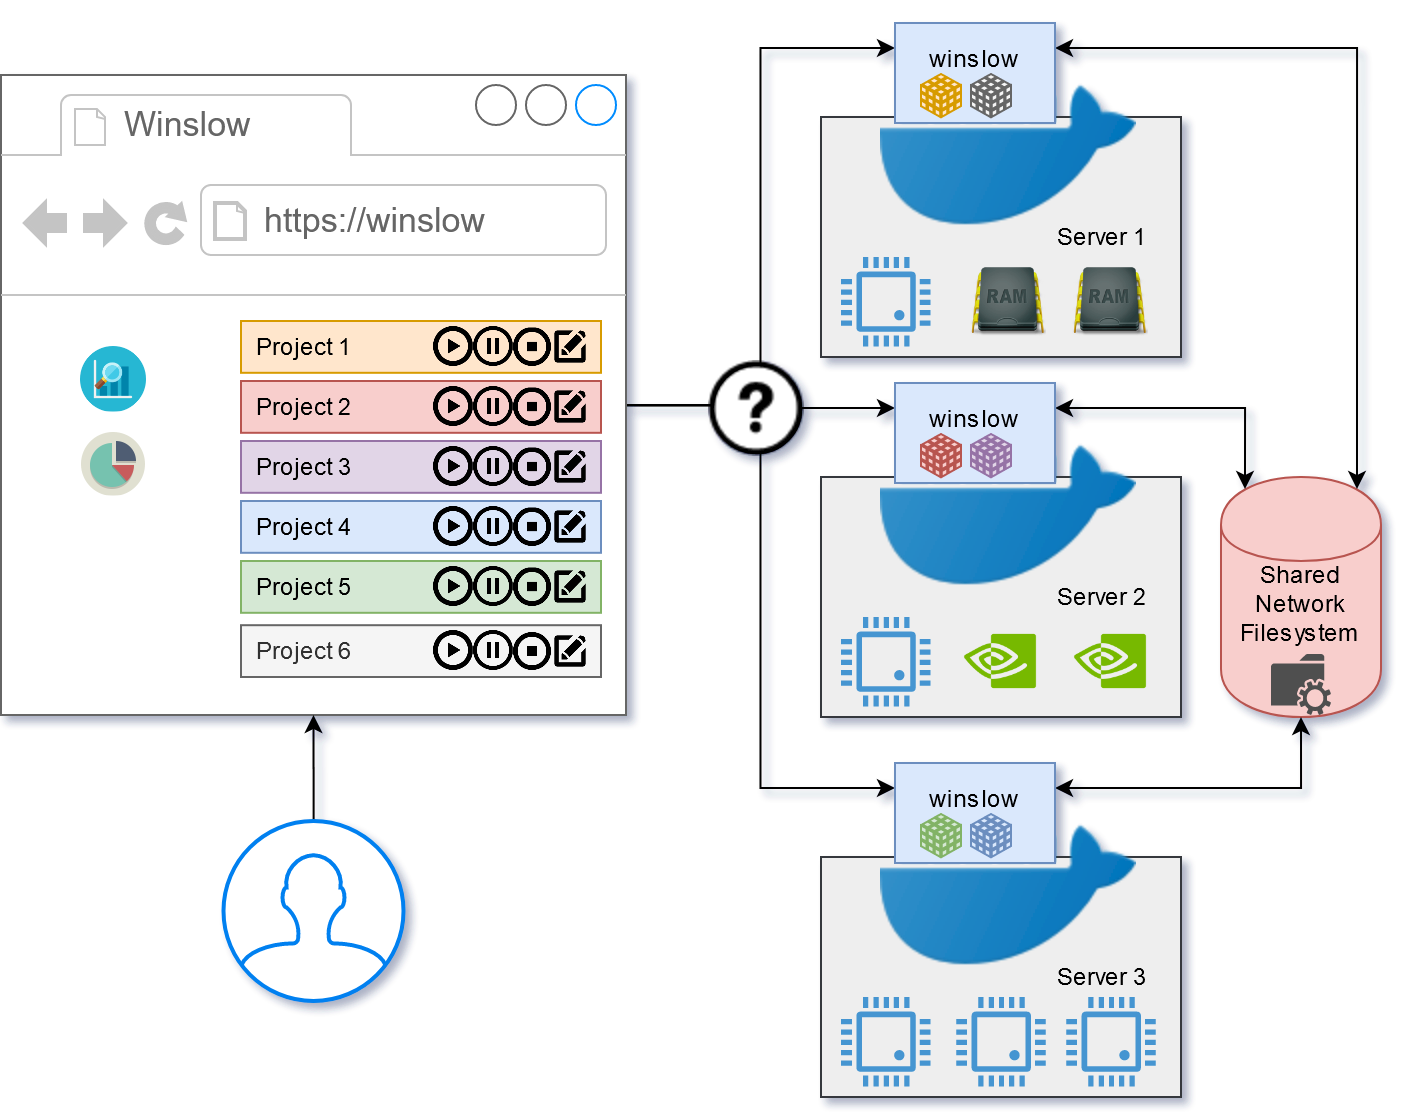
\includegraphics[width=0.8\textwidth]{architecture.png}
	\caption{High level view on the system structure}
	\label{architecture:high-level}
\end{figure}


\todo{explain what is going on in \autoref{architecture:high-level}}